\chapter{Estructura del espacio-tiempo 1/2}


	
\begin{tikzpicture}
	\fill [left color=red!50, right color=teal!50] (0,0) rectangle (6.5,.1);
	\fill [left color=teal!50, right color=blue!50] (6.5,0) rectangle (11.5,.1);
	\end{tikzpicture}

\vspace{10mm}
\begin{adjustwidth}{50pt}{50pt}
\begin{ejemplo}
\begin{figure}[H]
	\centering
	\includegraphics[width=1\textwidth]{imagenes/img30-01.png}
\end{figure}

Representación de los vectores de la base espacio-tiempo de un observador inercial que se mueve a velocidad constante respecto a nosotros, siguiendo escrupulosamente los principios de la relatividad especial.

El objetivo de este capítulo va a ser por qué es así y lo que esto significa.

\textcolor{gris}{Newton: Las leyes de la naturaleza son invariantes para cualquier observador inercial $\ \to \ $ Grupo de Galileo.}

\textcolor{gris}{Einstein: Las leyes de la naturaleza son invariantes para cualquier observador inercial $\ \to \ $ Grupo de Poincaré (para masas puntuales y para campos).}
\end{ejemplo}
\end{adjustwidth}
\vspace{5mm}

\section{Observador}

Un observador, o sistema de referencia, en física es el concurso de un punto fijo del espacio llamado origen y una base de tres vectores con una métrica que permita medir distancias y ángulos (`producto escalar'). Los vectores de la base los tomaremos ortonormales (mútuamente ortogonales, perpendiculares, y normalizados, de módulo unidad: $e_i \cdot e_j=\delta_{ij}$ ) $\left\{ \mathcal O; e_1, e_2, e_3 \right\}.$ Además, el sistema de referencia irá acompañado de un reloj, para la medida del tiempo.

\textbf{Producto escalar}: Asocia a cada pareja de vectores un número real y queremos que sea conmutativo $\ (\vec a \cdot \vec b=\vec b \cdot \vec a) \ $ y bilineal $\ ( \ (a+b)c=ac+bc;\ a(b+c)=ab+ac;\ (\lambda a)b=a(\lambda b)=\lambda(ab) \  )\ $, para ello escribimos:
$\quad \vec a \cdot \vec b=a^T \ \mqty(\text{matriz}\\ \text{métrica}) \ b \, , \ $ en dos dimensiones, $\ \mqty(a_1&a_2) \mqty(\alpha& \boldsymbol{\beta}\\ \boldsymbol{\beta} &\gamma) \mqty(b_1\\b_2)\, , \ $ la matriz métrica ha de ser simétrica por la condición de conmutatividad.

Para que se cumpla el teorema de Pitágoras,
\begin{multicols}{2}
\begin{figure}[H]
	\centering
	\includegraphics[width=.20\textwidth]{imagenes/img30-03.png}
\end{figure}

$\ h^2=c_1^2+c_2^2 \ \to  \ \mqty(c_1&c_2) \mqty(a&b\\b&c) \mqty(c_1\\c_2) \ \Rightarrow $

$\ a=c=1 \ ; \ b=0$ 
\end{multicols}
Luego la matriz métrica $g$ es la identidad: $\ g=I=\mqty(1&0\\0&1)$.

El origen del observador puede variar con el tiempo, $\mathcal O)t)$, el observador se mueve. Tambiñen podría ocurrir que los vectores básicos fuesen dependientes del tiempo, $\vec e_i=\vec e_i(t)$; pues bien definimos ...

\subsection{Observador inercial newtoniano}
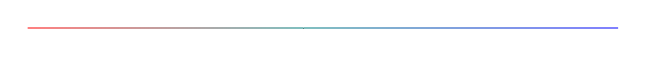
\begin{tikzpicture}
	\fill [left color=red!50, right color=teal!50] (0,0) rectangle (3.5,.01);
	\fill [left color=teal!50, right color=blue!50] (3.5,0) rectangle (7.5,.01);
	\end{tikzpicture}
	
Un observador inercial newtoniano es aquel observador en que la variación  $\mathcal O'(t)$ es lineal con $t$ y los vectores básicos no dependen del tiempo, $e_i\neq e_i(t)\, : \quad $ $\{ \ \mathcal O' \, (a+bt,c+dt,f+gt)\, ; e'_1,e'_2,e'_3\ \}$ 



\underline{Ejemplo} de observador inercial en $\mathbb R^2$: $\qquad \left\{  \mqty(2+3t\\1+t)\, ; \ e'_1=\dfrac 1 {\sqrt{2}} \mqty(1\\1)\, ,\   e'_2=\dfrac 1 {\sqrt{2}} \mqty(-1\\1) \right\}$

\vspace{5mm}
\begin{multicols}{2}
\begin{figure}[H]
	\centering
	\includegraphics[width=.5\textwidth]{imagenes/img30-04.png}
\end{figure}

$\{\mathcal O;\, e'_1,e'_2 \}$ es un observador inercial referido a nosotros $ \left\{ \mathcal O \mqty(0\\0);\, e_1=\mqty(1\\0), e_2=\mqty(0\\1) \right\} $ 

Medido por $\mathcal O \qquad Q=xe_1+ye_2$

Medido por $\mathcal O' \qquad Q=(2+3t)e_1+(1+t)e_2+x'e'1+y'e'_2 \ = \ x_1e_1+x_2e_2$
\end{multicols}

Como $\ e'_1=\dfrac 1{\sqrt{2}} \mqty(1\\1)=\dfrac 1{\sqrt{2}} (e_1+e_2) \ \text{ y } \ e'_2=\dfrac 1{\sqrt{2}} \mqty(-1\\1)=\dfrac 1{\sqrt{2}} (-e_1+e_2)$, tendremos


$(2+3t)e_1+(1+t)e_2+x'\left( \dfrac 1{\sqrt{2}} e_1 + \dfrac 1{\sqrt{2}} e_2 \right) + y' \left( -\dfrac 1{\sqrt{2}} e_1 + \dfrac 1{\sqrt{2}} e_2 \right)=x_1e_1+ye_2$

$\left(2+3t+\dfrac{x'}{\sqrt{2}}-\dfrac{y'}{\sqrt{2}} \right) e_1 +
\left(1+t+\dfrac{x'}{\sqrt{2}}+\dfrac{y'}{\sqrt{2}} \right) e_2 =xe_1+ye_2$

Luego, $\quad \begin{cases}
 \ 	2+3t+\dfrac{x'}{\sqrt{2}}-\dfrac{y'}{\sqrt{2}} &=x\\
 \ 	1+t+\dfrac{x'}{\sqrt{2}}+\dfrac{y'}{\sqrt{2}} &=y
 \end{cases}\, , \ $ matricialmente,
  $\quad \mqty(x\\y\\1) \ = \ \mqty(
 \dfrac 1{\sqrt{2}} &  -\dfrac 1{\sqrt{2}} & \vdots & 2+3t \\
  \dfrac 1{\sqrt{2}}&   \dfrac 1{\sqrt{2}} & \vdots & 1+t \\
  \cdots & \cdots & \cdot & \cdots \\
  0&0&\vdots &1
 ) \mqty(x'\\y'\\1)$

Siempre se obtienen resultados del tipo:

$\mqty(
r_{11}&r_{12}&\vdots&a+bt\\
r_{21}&r_{22}&\vdots&c+dt\\
\cdots &\cdots&\cdot&\cdots\\
0&0&\vdots&1
)\ \ $ con $\mqty(r_{11}&r_{12}\\r_{21}&r_{22})=R_2\ $ una matriz ortogonal: $RR^T=I$ (matriz de rotación).

En tres dimensiones tendremos:


$\mqty(
r_{11}&r_{12}&r_{13}&\vdots&a+bt\\
r_{21}&r_{22}&r_{23}&\vdots&c+dt\\
r_{31}&r_{32}&r_{33}&\vdots&d+et\\
\cdots &\cdots&\cdots&\cdot&\cdots\\
0&0&0&\vdots&1)\ \ $ matriz típica de transformación entre observadores inerciales.


Esquemáticamente, \hspace{2cm} $\qquad \boldsymbol{
\mqty(\ 
\boxed{ \mqty{ \\ & R_{3\times 3} & \\  \\ } } & \boxed{\mqty{ a+bt\\c+dt\\f+gt}} \\ \\
\boxed{\mqty{ 0&\ 0 \ &0 }} & \ \ \,  \boxed{\mqty{\,  &1&}\, }
\ \ \ )
}$


Si además introducimos la coordenada temporal $t=t'+m$, hay un tiempo inicial para $\mathcal O'$ (pero el tiempo transcurre del mismo modo, $\dd t= \dd t'$, tendremos $[ R=(r_{ij}) \ / \ RR^T=I ]\, $ :


$$\mqty(t\\ \cdots \\x\\y\\z\\\cdots\\1) \
\mqty(
1&\vdots& 0&0&0& \vdots & m\\
\cdots&\cdot&\cdots&\cdots&\cdots&\cdot&\cdots\\
0&\vdots&r_{11}&r_{12}&r_{13}&\vdots&a_1+b_1t\\
0&\vdots&r_{21}&r_{22}&r_{23}&\vdots&a_2+b_2t\\
0&\vdots&r_{31}&r_{32}&r_{33}&\vdots&a_3+b_3t\\
\cdots&\cdots&\cdots &\cdots&\cdots&\cdot&\cdots\\
0&\vdots&0&0&0&\vdots&1)\ \mqty(t'\\ \cdots \\x' \\y' \\z'\\ \cdots\\1) $$

Expresión que representa una \emph{transformación típica de Galileo completa}, describe como se ven las coordenadas espacio-temporales entre dos observadores inerciales, uno se mueve respecto del otro con velocidad constante.

Esquemáticamente,  $\qquad \qquad
\subrayado{\ 
\mqty(t\\ \cdots \\x\\y\\z\\\cdots\\1) \ 
\mqty(\ \ 
\boxed{\mqty{1}} & \boxed{\mqty{0&0&0)}} & \boxed{\mqty{\ \  m \ \ }}\\ \\
\boxed{\mqty{0\\0\\0}}&\boxed{ \mqty{ \\ & R_{3\times 3} & \\  \\ } } & \boxed{\mqty{ a+bt\\c+dt\\f+gt}} \\ \\
\boxed{\mqty{0}}&\boxed{\mqty{ 0&\ 0 \ &0 }} & \ \ \,  \boxed{\mqty{\,  &1&}\, }
\ \ \ )
\ = \ 
 \mqty(t'\\ \cdots \\x' \\y' \\z'\\ \cdots\\1)
 \ }$
\vspace{5mm}

Lo mejor de todo es que este tipo de transformaciones, este tipo de matrices, forman un \textbf{\emph{Grupo de Lie}} multiplicativo y continuo\footnote{ Ver, al menos, capítulo 1 del curso de `Grupos de Lie' de 	\emph{Javier García}. \\ Apuntes en \textcolor{blue}{https://github.com/igvaori/Grupos-de-Lie/blob/main/GRUPOS-DE-LIE.pdf?raw=true} }. Llamando $G$ a este tipo de matrices, $G_1\cdot G_2=G_3$, al multiplicar dos de estas matrices, la matriz resultante guarda la misma forma.



\begin{tiny}
\textcolor{gris}
{$\mqty(
1&\vdots& 0&0&0& \vdots & m\\
\cdots&\cdot&\cdots&\cdots&\cdots&\cdot&\cdots\\
0&\vdots&r_{11}&r_{12}&r_{13}&\vdots&a_1+b_1t\\
0&\vdots&r_{21}&r_{22}&r_{23}&\vdots&a_2+b_2t\\
0&\vdots&r_{31}&r_{32}&r_{33}&\vdots&a_3+b_3t\\
\cdots&\cdots&\cdots &\cdots&\cdots&\cdot&\cdots\\
0&\vdots&0&0&0&\vdots&1)  \mqty(
1&\vdots& 0&0&0& \vdots & m'\\
\cdots&\cdot&\cdots&\cdots&\cdots&\cdot&\cdots\\
0&\vdots&r'_{11}&r'_{12}&r'_{13}&\vdots&a'_1+b'_1t\\
0&\vdots&r'_{21}&r'_{22}&r'_{23}&\vdots&a'_2+b'_2t\\
0&\vdots&r'_{31}&r'_{32}&r'_{33}&\vdots&a'_3+b'_3t\\
\cdots&\cdots&\cdots &\cdots&\cdots&\cdot&\cdots\\
0&\vdots&0&0&0&\vdots&1)  =  \mqty(
1&\vdots& 0&0&0& \vdots & m''\\
\cdots&\cdot&\cdots&\cdots&\cdots&\cdot&\cdots\\
0&\vdots&r''_{11}&r''_{12}&r''_{13}&\vdots&a''_1+b''_1t\\
0&\vdots&r''_{21}&r''_{22}&r''_{23}&\vdots&a''_2+b''_2t\\
0&\vdots&r''_{31}&r''_{32}&r''_{33}&\vdots&a''_3+b''_3t\\
\cdots&\cdots&\cdots &\cdots&\cdots&\cdot&\cdots\\
0&\vdots&0&0&0&\vdots&1)$}
\end{tiny}

\begin{footnotesize}
$$\mqty(\ \ 
\boxed{\mqty{1}} & \boxed{\mqty{0&0&0)}} & \boxed{\mqty{\ \  m \ \ }}\\ \\
\boxed{\mqty{0\\0\\0}}&\boxed{ \mqty{ \\ & R_{3\times 3} & \\  \\ } } & \boxed{\mqty{ a+bt\\c+dt\\f+gt}} \\ \\
\boxed{\mqty{0}}&\boxed{\mqty{ 0&\ 0 \ &0 }} & \ \ \,  \boxed{\mqty{\,  &1&}\, }
\ \ \ ) \cdot \mqty(\ \ 
\boxed{\mqty{1}} & \boxed{\mqty{0&0&0)}} & \boxed{\mqty{\ \  m' \ \ }}\\ \\
\boxed{\mqty{0\\0\\0}}&\boxed{ \mqty{ \\ & R'_{3\times 3} & \\  \\ } } & \boxed{\mqty{ a'+b't\\c'+d't\\f'+g't}} \\ \\
\boxed{\mqty{0}}&\boxed{\mqty{ 0&\ 0 \ &0 }} & \ \ \,  \boxed{\mqty{\,  &1&}\, }
\ \ \ ) = \mqty(\ \ 
\boxed{\mqty{1}} & \boxed{\mqty{0&0&0)}} & \boxed{\mqty{\ \  m'' \ \ }}\\ \\
\boxed{\mqty{0\\0\\0}}&\boxed{ \mqty{ \\ & R''_{3\times 3} & \\  \\ } } & \boxed{\mqty{ a''+b''t\\c''+d''t\\f''+g''t}} \\ \\
\boxed{\mqty{0}}&\boxed{\mqty{ 0&\ 0 \ &0 }} & \ \ \,  \boxed{\mqty{\,  &1&}\, }
\ \ \ )$$
\end{footnotesize}


En mecánica newtoniana, toda ley ha de ser invariante baja transformaciones de Galileo que conecten dos observadores inerciales, ambos observadores describen las leyes del mismo modo.

La relatividad no es invariante bajo transformaciones de Galileo, lo es bajo transformaciones del grupo de Poincaré.

\vspace{5mm}

Veamos una \emph{sutileza} muy importante: estas transformaciones son para las coordenadas de puntos, el observador $\mathcal O'$ ve las coordenadas de $P(x'y')$ que el observador inercial con él $\mathcal O$ ve con coordenadas $P(x,y)$ dadas por

 $\quad \mqty(x\\y\\1) \ = \ \mqty(
 \dfrac 1{\sqrt{2}} &  -\dfrac 1{\sqrt{2}} & \vdots & 2+3t \\
  \dfrac 1{\sqrt{2}}&   \dfrac 1{\sqrt{2}} & \vdots & 1+t \\
  \cdots & \cdots & \cdot & \cdots \\
  0&0&\vdots &1
 ) \mqty(x'\\y'\\1)$

no ocurre así para las componentes de vectores. Si aplicásemos estas transformaciones a un vector obtendríamos la contradicción de que las componentes del nuevo vector varían con el tiempo y ello no es posible:

  $\quad \mqty(A_x\\A_y\\1) \ = \ \mqty(
 \dfrac 1{\sqrt{2}} &  -\dfrac 1{\sqrt{2}} & \vdots & 2+3t \\
  \dfrac 1{\sqrt{2}}&   \dfrac 1{\sqrt{2}} & \vdots & 1+t \\
  \cdots & \cdots & \cdot & \cdots \\
  0&0&\vdots &1
 ) \mqty(A'_x\\A'_y\\1) \ \to \ \begin{cases}
 \ A_x = \dfrac 1{\sqrt{2}} 	A'_x - \dfrac 1 {\sqrt{2}} A'y +2+3\boldsymbol{t} \\ 
 \ A_y=  \dfrac 1 {\sqrt{2}} A'_x + \dfrac 1 {\sqrt{2}} A'_y+ 1+\boldsymbol{t} 
 \end{cases}\ $ !`Imposible! 
 
 Para transformar vectores, la sutileza consiste en cambiar el $1$ por $0$ al final de los vectores columna:
 
  $\quad \mqty(A_x\\A_y\\ \boldsymbol{\textcolor{red}{0}}) \ = \ \mqty(
 \dfrac 1{\sqrt{2}} &  -\dfrac 1{\sqrt{2}} & \vdots & 2+3t \\
  \dfrac 1{\sqrt{2}}&   \dfrac 1{\sqrt{2}} & \vdots & 1+t \\
  \cdots & \cdots & \cdot & \cdots \\
  0&0&\vdots &1) \mqty(A'_x\\A'_y\\ \boldsymbol{\textcolor{red}{0}})\, , \ $ 
  
 es decir, los vectores solo se transforman con la submatriz ortogonal

  $\quad \mqty(A_x\\A_y) \ = \ \mqty(
 \dfrac 1{\sqrt{2}} &  -\dfrac 1{\sqrt{2}}  \\
  \dfrac 1{\sqrt{2}}&   \dfrac 1{\sqrt{2}} ) \mqty(A'_x\\A'_y) \ \to \ A=RA' \ \Rightarrow \    A'=R^{-1} A$
  
  $R$ matriz ortogonal (de rotación): $\ RR^T=I \leftrightarrow R^{-1}=R^T$

Galileo nos dice como cambiar un vector entre dos observadores inerciales y el sentido común nos dice que las leyes han de ser invariantes bajo estas transformaciones: $\ \vec F=m\vec a \leftrightarrow \vec F'=m\vec a'$, los vectores $\vec F$ y $\vec F'$ se expresarán con distintos números (los observadores verán que apuntan a distintas direcciones) pero ambos tendrán el mismo módulo (al igual que ocurrirá con $\vec a $ y $\vec a'$) por lo que las leyes serán invariantes bajo rotaciones.



\textcolor{gris}{Matrices de transformación entre observadores inerciales para las coordenadas de un punto y para las componentes de un vector.}

\begin{center}
\textcolor{gris}{
$\mqty(
r_{11}&r_{12}&r_{13}&\vdots&a+bt\\
r_{21}&r_{22}&r_{23}&\vdots&c+dt\\
r_{31}&r_{32}&r_{33}&\vdots&d+et\\
\cdots &\cdots&\cdots&\cdot&\cdots\\
0&0&0&\vdots&1)\quad 
\mqty(
r_{11}&r_{12}&r_{13}\\
r_{21}&r_{22}&r_{23}\\
r_{31}&r_{32}&r_{33}) \quad  \leftrightarrow \quad 
\boldsymbol{
\mqty(\ 
\boxed{ \mqty{ \\ & R_{3\times 3} & \\  \\ } } & \boxed{\mqty{ a+bt\\c+dt\\f+gt}} \\ \\
\boxed{\mqty{ 0&\ 0 \ &0 }} & \ \ \,  \boxed{\mqty{\,  &1&}\, }
\ \ \ )
}\quad  \mqty(\ \boxed{R_3}\ )
$}
\end{center}

\vspace{1cm}

\begin{example}

Ejemplo de \textbf{observador no inercial} en Newton.	




\begin{multicols}{2}
$\mathcal O\, ; e_1,e_2$ es un observador. $\mathcal O'\, ; e'_1(t),e'_2(t)$ es otro observador que está rotando sobre sí mismo, no es un observador inercial pues no se desplaza a $\vec v = \overrightarrow {cte}$ (respecto de $\mathcal O$) y las leyes de Newton no se expresarán del mismo modo para $\mathcal O$ y para $\mathcal O'$.

\vspace{2mm}Las leyes de la física solo serán invariantes para observadores inerciales, que se muevan a $\vec v = \overrightarrow {cte}$ pues, de este modo, resultan indistinguibles. 
\begin{figure}[H]
	\centering
	\includegraphics[width=.4\textwidth]{imagenes/img30-05.png}
\end{figure}	

\end{multicols}


\end{example}




\subsection{Observador inercial relativista}
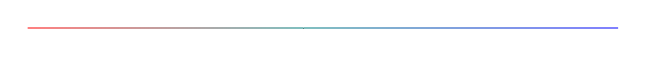
\begin{tikzpicture}
	\fill [left color=red!50, right color=teal!50] (0,0) rectangle (3.5,.01);
	\fill [left color=teal!50, right color=blue!50] (3.5,0) rectangle (7.5,.01);
	\end{tikzpicture}
	
Espacio-Tiempo: 1-dim espacial y 1-dim temporal. 

$\mathcal O\,: \ \  x^0=ct;\quad x^1=x\, ; \quad $ Para $\mathcal O':\ (ct',x')\, $ inercial respecto a $\mathcal O$

En nuestra representación, $\mathcal O'$ en el espacio, para él $x'=0$, solo le pasa el tiempo. En su línea de movimiento el vector unitario es $e'_0$. Así, $e'_1$ debería ser ortogonal respecto a $e'_0$ pero esto entra en contradicción con el principio de relatividad especial de Einstein en el que un rayo de luz debe ser visto a velocidad $\boldsymbol c$ para cualquier observador inercial.

Rayo de luz, $x=ct \to \vec c$ formará $45^o$ en el diagrama $t-x$	

Para $\mathcal O\,: \quad  \vec c \sim (1,1) \quad x=ct \ \to \ \Delta x=c\Delta t$

Según el principio de relatividad, para $\mathcal O'\,: \vec c \sim (1,1)$ también, componentes iguales para que de la misma velocidad.

Por esto, el vector $e'_1$ es el que aparece en la figura como  \textcolor{blue}{$e'_1$} y no puede ser el que aparece como \textcolor{blue}{$\cancel{e'_1}$}. Ha de ser simétrico a $e'_0$ respecto de la dirección del rayo de luz, respecto de la bisectriz del primer y tercer cuadrantes)
	
	
\begin{figure}[H]
	\centering
	\includegraphics[width=.95\textwidth]{imagenes/img30-06.png}
\end{figure}	
	
La métrica aún no sabemos como debe ser, $\ g=\mqty( g_{00} & g_{01} \\ g_{10} & g_{11} )\, , \  $ pero como los vectores básicos han de ser ortonormales $\ \to \ e_{0}\cdot e_{1}=0\ $ y también para el otro observador inercial, $\ e_{0'}\cdot e_{1'}=0\ $ además $\ e_{0'}\cdot e_{0'}=e_{0}\cdot e_{0} \ $ y  $\ e_{1'}\cdot e_{1'}=e_{1'}\cdot e_{1'}\ $, no puede haber distinción entre dos observadores inerciales, por lo que $\ g_{01}=g_{10}=0$
	
	
$e_o\cdot e_1=\mqty(\alpha & 0)\mqty( g_{00} & g_{01} \\ g_{10} & g_{11} )\mqty(0\\ \beta)=\mqty(\alpha & 0) \mqty(g_{01}\beta \\ g_{11} \beta)=\alpha g_{01} \beta = 0 ,\ \forall \alpha, \forall \beta \ \Rightarrow \ g_{01}=0 $
	
	
Como el producto escalar es conmutativo, $\ \vec a \cdot \vec b=\vec b \cdot \vec a \ \to \ g_{10}=g_{01}=0$	

Si $e_{0'}=ae_0+be_1$, como $e_{1'}$ ha de ser su simétrico respecto de la línea de $45^o$ (bisectriz), no quesa más remedio que intercambiar componentes y $e_{1'}=be_0+ae_1$

Como $e_{0'}\cdot e_{1'}=0 \to (ae_0+be_1)\cdot (be_o+ae_1)=abe_0e_0+0+0+bae_1e_1=abg_{00}+bag_{11}=ab(g_{00}+g_{11})=0,\ \forall a,\, \forall b \ \Rightarrow \ g_{00}=-g_{11}$

Si además $e_0\cdot e_0=1 \ \to\ g_{00}=1 \ \to \ g_{11}=-1$

Y la matriz métrica espacio temporal será: $\quad \boldsymbol{\mqty(1&0\\0&-1)}$

\begin{small}
\textcolor{gris}{	
Cualquier observador inercial se puede ver como un sistema de referencia en el que ese observador, con respecto al sistema de referencia enganchado a sí mismo, siempre tendrá componente $x'=0$ y la única dimensión libre será la del tiempo. Por ello hemos puesto $e'_0$ en el eje del movimiento del observador. De ahí, $e'_1$ ha de ser  simétrico respecto a la bisectriz, debido al primer principio de la relatividad que dice que la velocidad de la luz ha de ser constante.}

\textcolor{gris}{Al poder distinguir entre qué es moverse por el espacio y qué es moverse por el tiempo (dimensiones independientes), hemos llegado a que $e_0	 \cdot  e_1=0$.}

\textcolor{gris}{También hemos usado el segundo postulado de la relatividad diciendo que ha de ocurrir lo mismo en cualquier sistema de referencia inercial, por lo que $e'_0 \cdot e'_1=0$.}

\textcolor{gris}{Por último, geométricamente hemos averiguado la relación entre las componentes de la métrica $g_{00}=-g_{11}$.}
\end{small}		

\vspace{5mm}	
\begin{figure}[H]
	\centering
	\includegraphics[width=.75\textwidth]{imagenes/img30-07.png}
\end{figure}	

Nos proponemos encontrar como se escriben los vectores $e'_0$ y  $e'_1$ respecto a  $e_0$ y  $e_1$, queremos expresarlo en función de la velocidad $v$ con que se desplaza $\mathcal O'$ respecto de $\mathcal O$.
	
$e'_0=f(v)e_0+g(v)e_1 \ \Rightarrow \text{ si } \ v \to 0 \ \Rightarrow \ \begin{cases}
 \ f(v)\to 1 \\ \ g(v) \to 0	 \end{cases} \quad \text{así } \ e'_0=e_0 \text{ con } v \to  0$ 
 
 Por simetría (bisectriz), $\ e'_1=g(v)e_0+f(v)e_1 \ \text{ y se cumple } \ 
\begin{cases}
 \ f(v)\to 1 \\ \ g(v) \to 0	 \end{cases} \quad \text{así } \ e'_1=e_1 \text{ con } v \to  0$	
 
 Además, $e'_o \cdot e'_1=0$
 
 Sabemos que $\ e'_0\cdot e'_0=g_{0'0'}=\textit{(obs. inerciales)}=g_{00}=1$, por lo que
 
 $1= e'_0\cdot e'_0=(fe_0+ge_1)\cdot (fe_0+ge_1)=f^2\cdot 1 + 0 + 0 + g^2 \cdot (-1)=\boldsymbol{ f^2-g^2=1}$
 
 Si exigimos $e'_1\cdot e'_1=g_{1'1'}=g_{11}=-1 \to g^2-f^2=-1$, que es la misma condición que la anterior.
 
 Tenemos la condición, $\ \boldsymbol{ f^2-g^2=1}$, condición que se cumple, por ejemplo, si hacemos $f=\cosh \theta$ y $g=\sinh \theta$, con $\theta=\theta(v)\ $ ya que $\ \cosh^2 \theta - \sinh^2 \theta=1\, , \ $ así que
$\ \ \begin{cases} \ e'_0=\cosh \theta + \sinh \theta \\ \ e'_1=\sinh \theta + \cosh \theta \end{cases}$
	
Tenemos que comprobar que se cumple que 	$\ \text{ si } \ v \to 0 \ \Rightarrow \ \begin{cases}
 \ f(v)\to 1 \\ \ g(v) \to 0	 \end{cases} \, . \ $ 
 
 Efectivamente, $ \ \text{ si } \theta \to 0 \ \Rightarrow \ \begin{cases} \ \cosh \theta \to 0 \\ \ \sinh \theta \to 0 \end{cases}$
 
 Vamos a encontrar cual es la relación $\theta=\theta(v)$, para ello sabemos que cualquier punto del espacio tiempo es de la forma $ct \ e_0+x\ e_1$, para $\mathcal O'$ este mismo punto será $ct' \ e'_0+x'\ e'_1$ y usando las expresiones anteriores,
 
 $ct \ e_0+x\ e_1 = ct'\ (\cosh \theta \ e_0 + \ \sinh \theta \ e_1) \ + \ x'\ ( \sinh \theta \ e_0 + \cosh \theta \ e_1) =$
 
$= (ct' \cosh \theta + x' \sinh \theta) \ e_0 \ + \ (ct' \sinh \theta +x' \cosh \theta) \  e_1  \ \to \ \begin{cases} \ ct=ct' \cosh \theta + x'\sinh \theta \\ \ x=ct' \sinh \theta + x' \cosh \theta \end{cases}$
	 
	
Matricialmente, $\quad \mqty(ct\\x) = \mqty(\cos h \theta & \sin h \theta \\ \sinh \theta & \cosh \theta) \mqty(ct'\\x')$

Si $\mathcal O'$ está en el origen de coordenadas y para él solo pasa el tiempo, $x'=0$ que llevado a la relación anterior,
$\quad \mqty(ct\\x) = \mqty(\cos h \theta & \sin h \theta \\ \sinh \theta & \cosh \theta) \mqty(ct'\\0) \ \to \ \begin{cases} \ ct=\cosh \theta \ ct' \\ \ x=\sinh \theta \ x' \end{cases}$, relaciones que dividiéndolas nos dan la relación $\quad \boldsymbol{\dfrac 1 c \dfrac x t = \tanh \theta}$

El observador $\mathcal O'$, que permanece quieto respecto de su sistema de referencia que lleva enganchado ($x'=0$), es visto por nosotros, observador $\mathcal O$, de manera que se mueve con velocidad $\ \dfrac x t =c \tanh \theta  = v$, por lo que la relación que buscábamos $\theta=\theta(v)$ es $\boldsymbol{ \theta=\mathrm{arctanh} \left( \dfrac v c \right) }$
	
Como $\cosh^2 \theta -\sinh^2 \theta=1$ y $\tanh \theta=\dfrac {\sinh \theta}{\cosh \theta}=\dfrac v c =\beta$, entonces
	
\textcolor{gris}{$sh=\beta \ ch \ \to \ c^2-(\beta \ ch)^2=1 \ \to \ (1-\beta)^2 \ ch = 1 \ \to \ $} $\cosh \theta = \dfrac 1{\sqrt{1-\beta^2}}=\gamma$ y también \textcolor{gris}{$sh=th\ ch =\beta \ ch\ \to \ $} $\sinh \theta = \gamma \beta $

\vspace{5mm}
\begin{large}
\begin{myblock}{Boost de Lorentz}
\begin{equation}
\label{T30boostLorentz}
\boldsymbol{
\mqty(ct\\x) \ = \ \mqty(\gamma & \gamma \beta \\ \gamma \beta & \gamma ) \mqty(ct'\\x')
\quad \Leftrightarrow \quad
\mqty(ct'\\x') \ = \ \mqty(\gamma & -\gamma \beta \\ -\gamma \beta & \gamma ) \mqty(ct\\x)
}	
\end{equation}
\end{myblock}
\end{large}
\vspace{5mm}

\color{gris}
La segunda de las transformaciones es la inversa de la primera, es muy sencillo comprobar que 

$\mqty(\gamma & \gamma \beta \\ \gamma \beta & \gamma)^{-1}=\mqty(\gamma & -\gamma \beta \\ -\gamma \beta & \gamma) \quad $ o que $\quad \mqty(\cos h \theta & \sin h \theta \\ \sinh \theta & \cosh \theta)^{-1}=\mqty(\cos h \theta & -\sin h \theta \\ -\sinh \theta & \cosh \theta)$, 

como vimos al final del capítulo anterior.

\color{black}
Estas transformaciones se llaman boost (movimiento relativo entre dos observadores) de Lorentz. \textcolor{gris}{En el siguiente capítulo veremos las rotaciones y las traslaciones.}

En el capítulo anterior obtuvimos el boost de Lorentz de un modo forzado, exigiendo no sabemos por qué, que $\partial_\mu \phi \partial^\mu \phi$ fuese invariante. Ahora lo hemos obtenido tan solo como derivación de los postulados de la teoría de la relatividad especial.


\vspace{5mm}
\begin{example}

Ejemplo de \textbf{observador no inercial} en relatividad especial.	

Un observador inercial en relatividad especial será cualquier observador que no se mueva en línea recta en el diagrama espacio-tiempo, $t-x$
\begin{multicols}{2}
 $v_0<v_1<v_2$. En $v_0\approx 0$ coinciden los vectores $e'_0$ y $e'_1$ con los $e_0$ y $e_1$ 
 
 A medida que aumenta la velocidad, los vectores $e'_0$ y $e'_1$ se van acercando uno al otro, el ángulo de separación entre ellos se hace más pequeño, que era lo que observábamos en la introducción del tema.
\begin{figure}[H]
	\centering
	\includegraphics[width=.4\textwidth]{imagenes/img30-08.png}
\end{figure}	

\end{multicols}

\end{example}





